\def\QRCODE{TB_image_TUT.IMG.image_restoration_denoising_matlabqrcode.png}
\def\QRPAGE{http://www.iptutorials.science/tree/master/TB_image/TUT.IMG.image_restoration_denoising/matlab}
\def\difficulty{2}
\mcorrectionsection{Matlab correction}


\subsection{Generation of random noises}
In order to convert the images into 8bits unsigned variables, the following function can be used:

\begin{matlab}
function A=hist_stretch(B)
% histogram stretching.
% ensure the range is [0; 255]
A = B - min(B(:));
A = 255 * A / max(A(:));
A = uint8(A);
\end{matlab}

In order to display the results in Figs.\ref{fig:image_restoration_denoising:matlab:noises} and \ref{fig:image_restoration_denoising:matlab:histograms}, a size $S=32$ will be used to generate the noisy images.
\begin{figure}[htbp]
 \centering
 
 \subfloat[Uniform noise.]{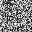
\includegraphics[width=.4\linewidth]{uniform_noise.png}}
 \hspace{1cm}
 \subfloat[Gaussian noise.]{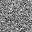
\includegraphics[width=.4\linewidth]{gaussian_noise.png}}
 
  \subfloat[Salt and pepper noise.]{
\includegraphics[width=.4\linewidth]{sp_noise.png}} \hspace{1cm}
 \subfloat[Exponential noise.]{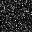
\includegraphics[width=.4\linewidth]{exp_noise.png}}

 \caption{Resulting noise images.}
 \label{fig:image_restoration_denoising:matlab:noises}
\end{figure}

\subsubsection{Uniform noise}
The \matlabregistered{} \minline{rand} function generates values between 0 and 1 with uniform distribution.

\begin{matlab}
S=32; a=0; b=255;
R1=a+(b-a)*rand(S);
\end{matlab}

\subsubsection{Gaussian noise}
The \matlabregistered{} \minline{randn} function generates values with normal centered distribution.
\begin{matlab}
a=0; b=1;
R2=a+b*randn(S);
R2=hist_stretch(R2);
\end{matlab}

\subsubsection{Salt and pepper noise}
\begin{matlab}
a=0.05;b=0.05;
R3=0.5*ones(S);
X=rand(S);
R3(X<=a)=0;
R3(X>a & X<=a+b)=1;
R3=hist_stretch(R3); 
\end{matlab}


\subsubsection{Exponential noise}
\begin{matlab}
a=1;
R4=-1/a*log(1-rand(S));
R4=hist_stretch(R4); 
\end{matlab}

\begin{figure}[htbp]
 \centering
 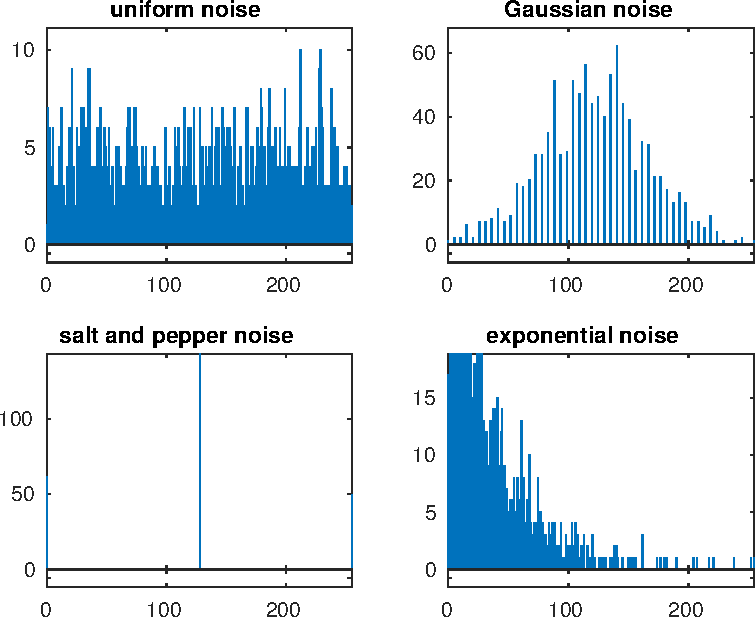
\includegraphics[width=\textwidth]{histograms_noise.pdf}
 \caption{Histograms of the noise images generated with $32\times 32$ pixels.}
 \label{fig:image_restoration_denoising:matlab:histograms}
\end{figure}


\subsection{Noise estimation}
In order to estimate the noise, a ROI of visually constant gray level is chosen, and its histogram is displayed. This is simulated by the following code, the result is displayed in Fig.\ref{fig:image_restoration_denoising:matlab:histogram_roi}:

\begin{matlab}
A=imread('jambe.tif');
A=double(A);
A=A/255;
c=[160 200 200 160];
r=[200 200 240 240];
C=roipoly(A,c,r);
imhist(A(C));

% exponential noise
[m,n]=size(A);
expnoise=1/0.5*log(1-rand(m,n));
B=A-expnoise/max(abs(expnoise(:)));B=hist_stretch(B);
imwrite(B, 'im_exp.png');
figure;
subplot(1,2,1);viewImage(B);title('Image with exponential noise');
subplot(1,2,2);imhist(B(C));title('histogram in ROI');

% Gaussian noise
B=imnoise(A,'gaussian',0,0.004);
imwrite(B, 'im_gauss.png');
figure;
subplot(1,2,1);viewImage(B);title('image with Gaussian noise');
subplot(1,2,2);imhist(B(C));title('histogramin ROI');
\end{matlab}

\begin{figure}[htbp]
\centering
\subfloat[ROI.]{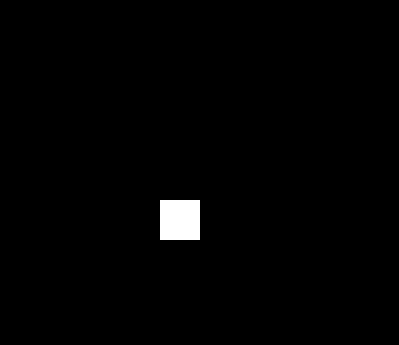
\includegraphics[height=.4\linewidth]{roi.png}} \hfill
\subfloat[Histogram.]{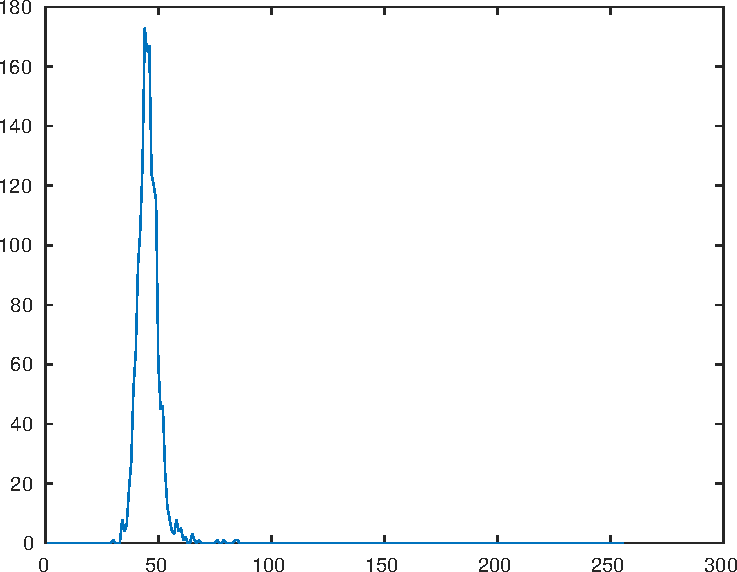
\includegraphics[height=.4\linewidth]{histogram_roi.pdf}}
 \caption{Histogram of the Region of Interest.}
 \label{fig:image_restoration_denoising:matlab:histogram_roi}
\end{figure}

In the case of exponential and Gaussian noise added to the image, The histograms are displayed in Figs.\ref{fig:image_restoration_denoising:matlab:hist_exp} and \ref{fig:image_restoration_denoising:matlab:hist_gauss}.

\begin{figure}[htbp]
 \centering
 \subfloat[Addition of exponential noise to the original image of the leg.]{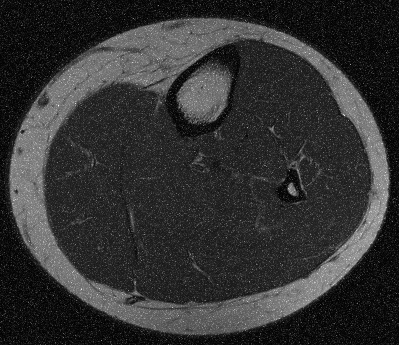
\includegraphics[height=.4\linewidth]{im_exp.png}}\hfill
  \subfloat[Histogram of the ROI.]{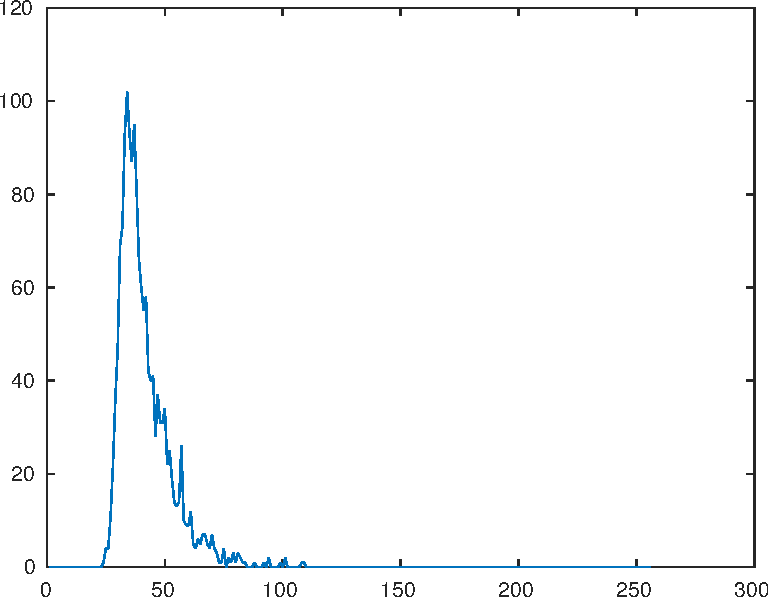
\includegraphics[height=.4\linewidth]{hist_exp.pdf}}

  \caption{Exponential noise.}
  \label{fig:image_restoration_denoising:matlab:hist_exp}
\end{figure}

\begin{figure}[htbp]
 \centering
 \subfloat[Addition of Gaussian noise to the original image of the leg.]{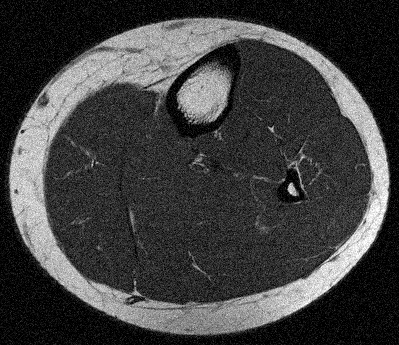
\includegraphics[height=.4\linewidth]{im_gauss.png}}\hfill
  \subfloat[Histogram of the ROI.]{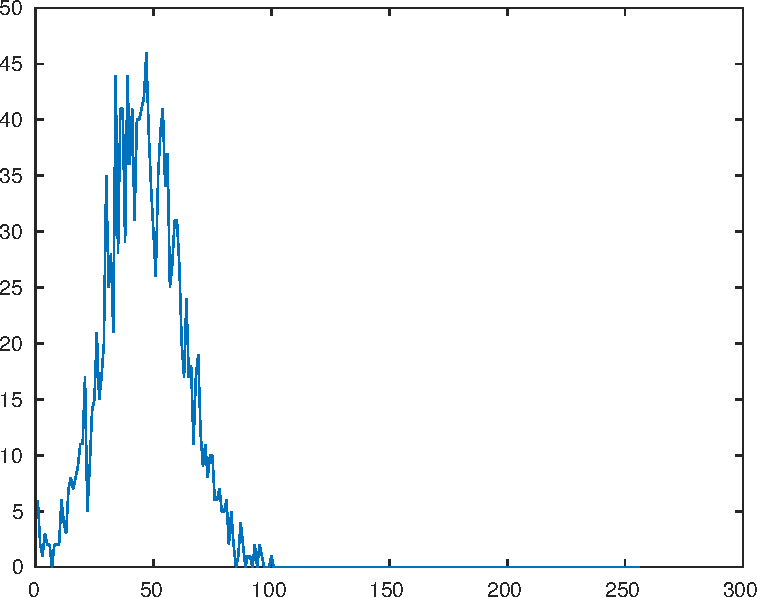
\includegraphics[height=.4\linewidth]{hist_gauss.pdf}}

  \caption{Gaussian noise.}
  \label{fig:image_restoration_denoising:matlab:hist_gauss}
\end{figure}

\newpage
\subsection{Image restoration by spatial filtering}
The following code is used to filter the images. The results are displayed in Fig.\ref{fig:image_restoration_denoising:matlab:filters}.
\begin{matlab}
A=imread('jambe.tif');
A=double(A);
A=A/255;
[m,n]=size(A);
% add salt and pepper noise
B=imnoise(A,'salt & pepper', 0.25);
% filtering
% mean
w=fspecial('average',5);
B1=imfilter(B,w);
% max
B2=ordfilt2(B,9,ones(3,3));
% min
B3=ordfilt2(B,1,ones(3,3));
% median
B4=medfilt2(B,[7,7]);
\end{matlab}

\begin{figure}[htbp]
 \centering
 \subfloat[Original image.]{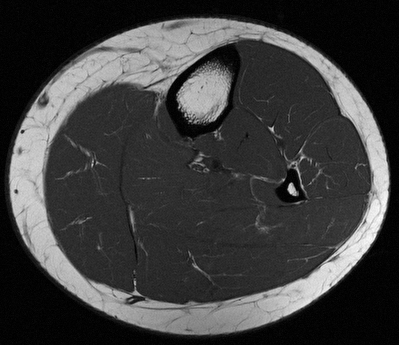
\includegraphics[width=.4\linewidth]{jambe.png}}
 \hspace{1cm}
 \subfloat[Noisy image (salt and pepper).]{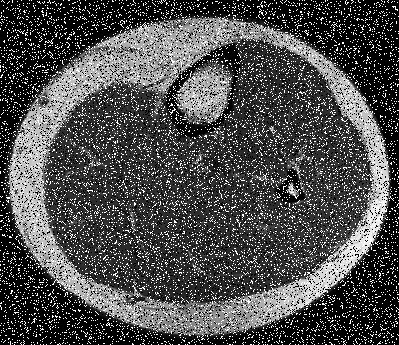
\includegraphics[width=.4\linewidth]{noise_image.png}}
 
 \subfloat[Maximum filter.]{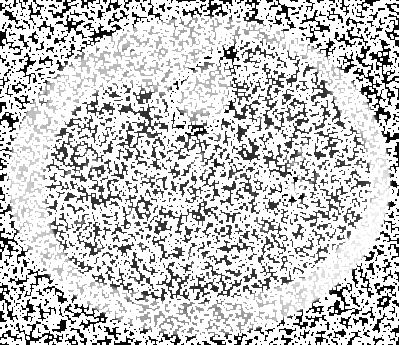
\includegraphics[width=.4\linewidth]{max_filter.png}}
 \hspace{1cm}
 \subfloat[Minimum filter.]{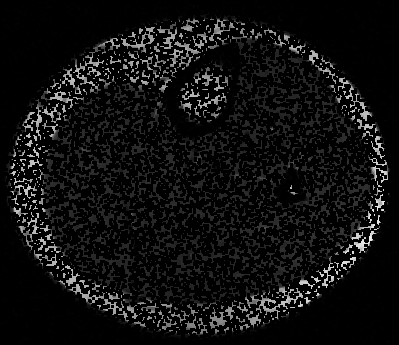
\includegraphics[width=.4\linewidth]{min_filter.png}}
 
 \subfloat[Mean filter.]{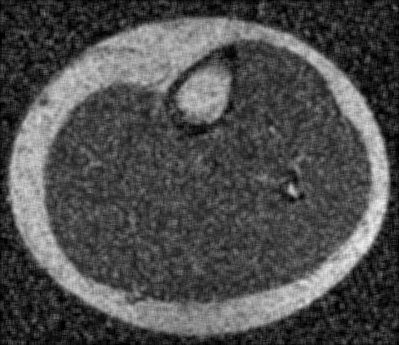
\includegraphics[width=.4\linewidth]{mean_filter.png}}
 \hspace{1cm}
 \subfloat[Median filter.]{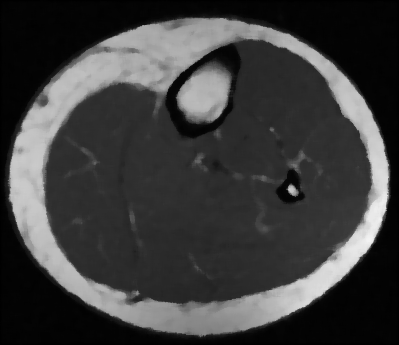
\includegraphics[width=.4\linewidth]{med_filter.png}}
 
 \caption{Different filters applied to the noisy image. The median filter is particularly adapted in the case of salt and pepper noise (impulse noise), but still destroy the structures observed in the images.}
 \label{fig:image_restoration_denoising:matlab:filters}

\end{figure}

What can be noticed is that min and max filters are unable to restore the image (opening and closing filters, from the mathematical morphology, could be a solution to explore). The mean filter is a better solution, but an average value is highly modified by an impulse noise. The median filter is the optimal solution is order to suppress the noise, but fine details are lost. An interesting solution is to apply an adaptive median filter. 

\newpage
\subsubsection{Adaptive median filter}
The following code is a simple implementation of the algorithm previously presented. It has not been optimized in order to have a simple presentation. A more sophisticated version can be found in \cite{Gonzalez2002}. The results are illustrated in Fig.\ref{fig:image_restoration_denoising:matlab:amf_filter} for $S_{max}=7$.

\begin{matlab}
function f = amf(I, Smax)
% adaptive median filter
% I: original image
% Smax: size maxi of neighborhood

f = I;

sizes=1:2:Smax;
zmin = zeros([size(I) length(sizes)]);
zmax = zeros([size(I) length(sizes)]);
zmed = zeros([size(I) length(sizes)]);

for k=1:length(sizes),
    zmin(:,:,k) = ordfilt2(I, 1, ones(sizes(k)), 'symmetric');
    zmax(:,:,k) = ordfilt2(I, sizes(k)^2, ones(sizes(k)), 'symmetric');
    zmed(:,:,k) = medfilt2(I, [sizes(k) sizes(k)], 'symmetric');
end

% determines for all scales at the same time if zmed is an impulse noise.
% this enables the choice of the scale.
isMedImpulse = (zmin==zmed) | (zmax==zmed);

for i=1:size(I,1)
    for j=1:size(I,2)
        
        % finds the right scale
        % determines k (neighborhood size) where the median value is not an
        % impulse noise
        k=1;
        while isMedImpulse(i,j,k) && k<length(sizes)
            k = k+1;
        end
        
        % if the value of the pixel I(i,j) is an impulse noise, it is
        % replaced by the median value at scale k, if not, it is kept
        % untouched (already set)
        if I(i,j)==zmin(i,j,k) || I(i,j)==zmax(i,j,k) ||  k == length(sizes)
            f(i,j) = zmed(i,j,k);
        end

    end
end
\end{matlab}

\begin{figure}[htbp]
 \centering
 
 \subfloat[Original image.]{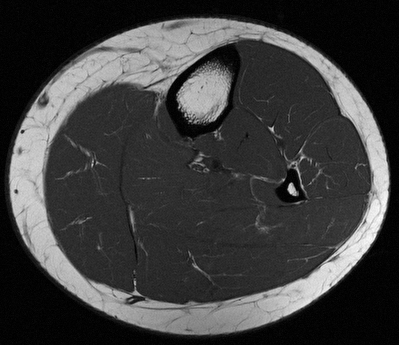
\includegraphics[width=.4\linewidth]{jambe.png}}
 \hspace{1cm}
 \subfloat[Noisy image (salt and pepper).]{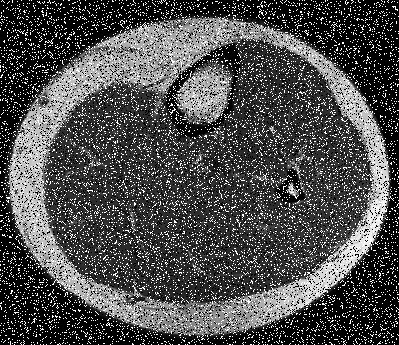
\includegraphics[width=.4\linewidth]{noise_image.png}}
 
 \subfloat[Median filter of size $7\times 7$.]{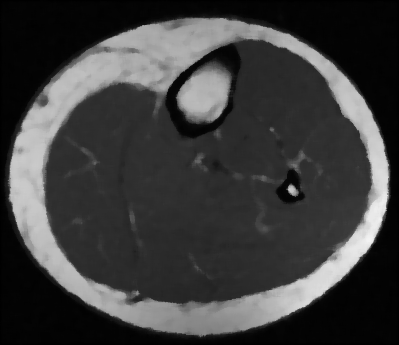
\includegraphics[width=.4\linewidth]{med_filter.png}}
 \hspace{1cm}
 \subfloat[Adaptive median filter, $S_{max}=7$.]{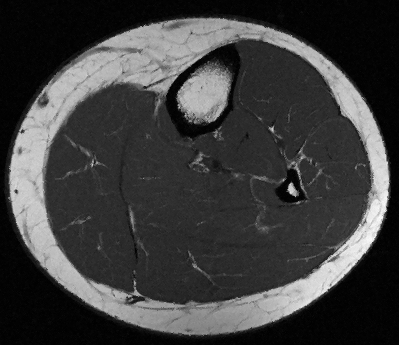
\includegraphics[width=.4\linewidth]{amf_filter.png}}

 \caption{Illustration of the adaptive median filter.}
 \label{fig:image_restoration_denoising:matlab:amf_filter}
\end{figure}
